\chapter{Evaluation} 

\section{Controlled Movements}
\label{sec:controlled_movements}

% Comparison deadreckoning accuracy of battery powered robot with solar powered robot

% Try at least one more supercapacitor: 10mF
% Study reducing the frequency of power interrupts ie smaller energy buffer.
% How does this effect the accuracy of locomotion?
% Can the frequency of power interrupts be related to the 

% Video of robot movement

In this section the accuracy of movement of the battery-less robot and its battery powered counterpart will be compared.

\subsection{Experimental setup}

To be able to compare the accuracy of the robot while it is exposed to increasingly smaller power cycles, a variety of movements is recorded using a overhead camera.
A camera stand with DSLR camera is positioned on a tabletop and in the camera's view the corners of a square of 80$\times$80\,cm are indicated with a black marker, see Figure \ref{fig:movement_setup}.
This square is later used as a reference to convert the robots movement from pixels to cm.
Three different movements are compared, while the robot is moving straight movement of 75\,cm, a circle with radius of 30 cm and a square of 50$\times$50\,cm.

\subsubsection{Artificial Power Interrupts}

%TODO Why bat powered
During the experiment the robot will be powered from a battery and power interrupts, i.e the capacitor running out of energy are created artificially using a timer that resets the MCU.
The MSP430FR5969 has the functionality to enable a brownout reset trough software which is used to simulate the event of the supply voltage dropping below the required operating voltage.
With a capacitor of 22\,mF the robot can operate around 1 second, this resulted in the chosen interrupt periods.
Choosing a period smaller than half a second resulted in uncontrolled behavior, while the control loop was not able to stabilize the movement before the robot runs out of energy again.
Therefore the power interrupt periods evaluated in this experiment were set to th value above and equal to 0.5\,s: 1.25\,s, 1\,s, 0.75\,s and 0.5\,s.

\subsubsection{Velocity Calibration}

%TODO make table with standard deviation of distance traveled 
Each movement is executed at three different velocity PWM target settings: 40\%, 65\% and 90\% of the maximum duty cycle.
To let the robot move a particular distance, the average speed needs to be estimated for each PWM target and power interrupt period.
This is achieved by first determining the time that the robot requires to move approximately 150\,cm for each target without power interrupts.
When the robot experiences power interrupts the average velocity of a active period becomes lower due to frequent acceleration from a standstill.
With power interrupts the runtime is increased to make the robot travel roughly the same distance.
Finally, the average of five complete movement measurements is computed and divided by the commanded runtime of the robot to acquire an average speed for each combination, which can be found in Table \ref{tab:val_calib}.


\begin{table}[t]
	\centering
	\small
	\caption{Calibrated velocity}
	\label{tab:val_calib}
	\begin{tabular}{|l|l|l|l|l|l|}
		\hline
		& No int & 1.25\,s & 1.0\,s & 0.75\,s & 0.5\,s \\
		\hline \hline
		Target 40\% & 18.9\,m/s & 18.2\,cm/s & 18.0\,cm/s & 17.1\,cm/s & 15.9\,cm/s \\
		Target 65\% & 24.0\,m/s & 22.2\,cm/s & 21.3\,cm/s & 20.8\,cm/s & 18.8\,cm/s \\
		Target 90\% & 28.8\,m/s & 26.4\,cm/s & 25.7\,cm/s & 24.5\,cm/s & 22.7\,cm/s \\
		\hline
	\end{tabular}
\end{table}

\subsubsection{Tracking the Movement}

The robot is programmed to preform the movement at a desired PWM target ie at a specified speed, and optional power interrupt period.
Before the robot executes the movement a green led is enabled on top of the robot.
This green dot will be the reference point that the tracking software will try to follow.
The camera is used to record the movement which then is analyzed using Python and OpenCV 3.2.
An example of a tracked movement can be seen in Figure \ref{fig:movement_example}.

\begin{figure}
	\centering
	\begin{subfigure}[b]{0.45\textwidth}
		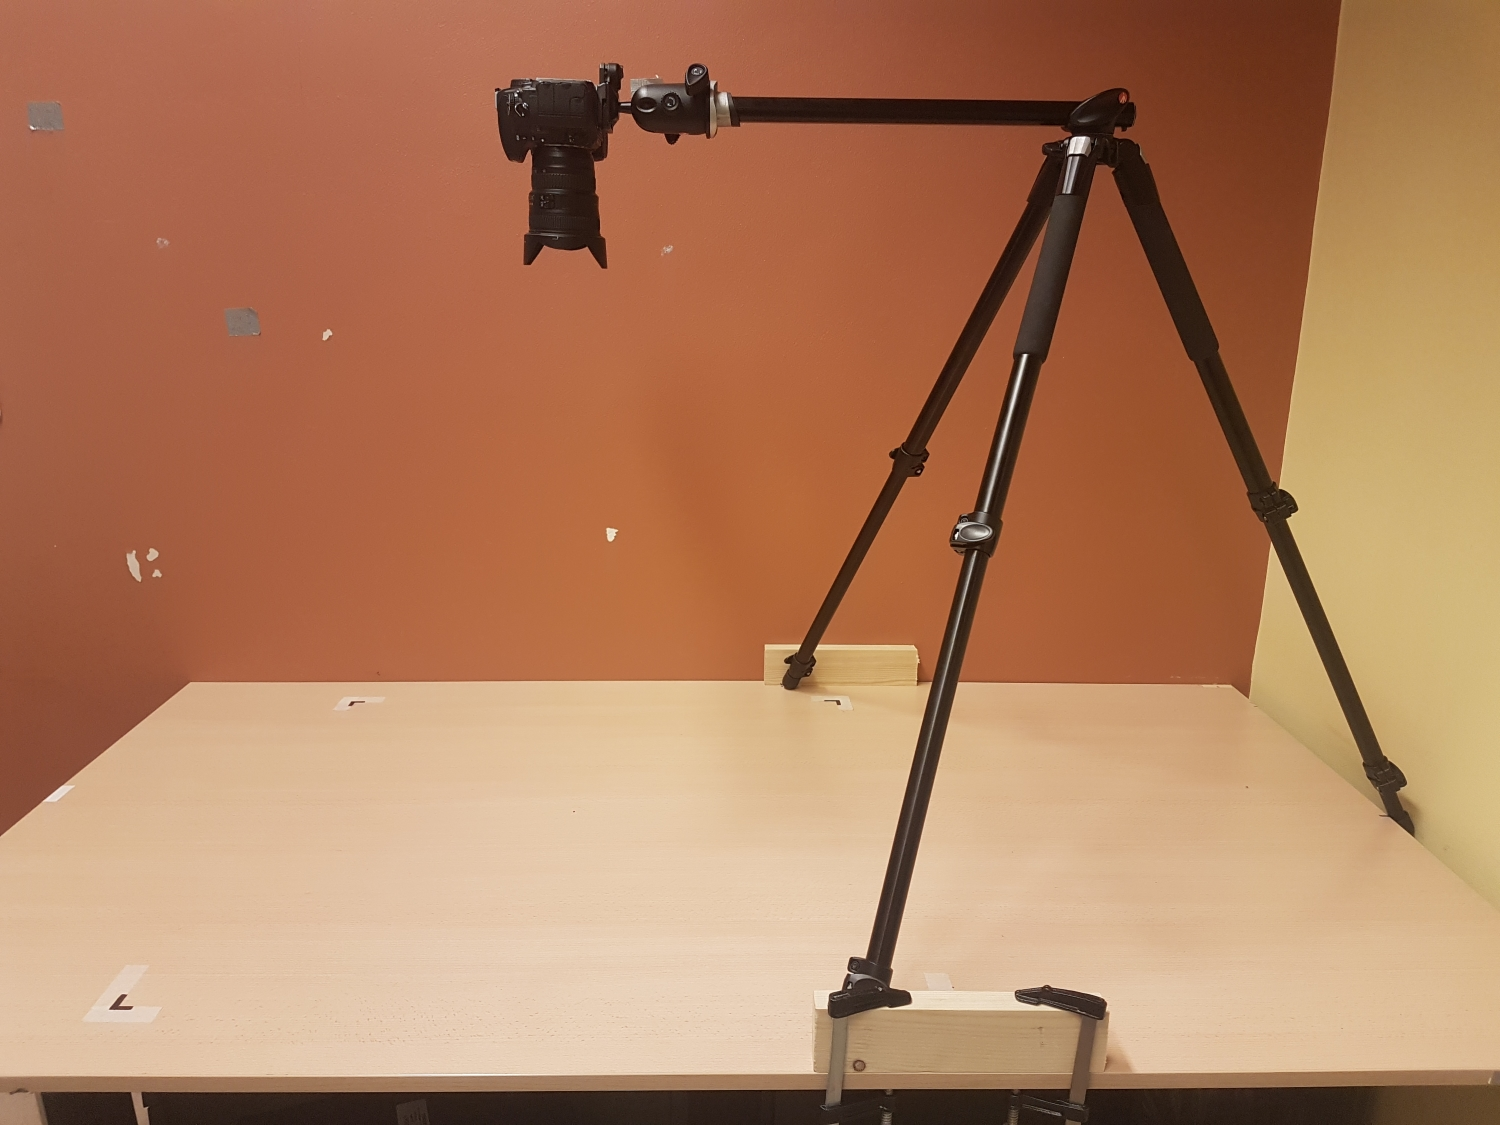
\includegraphics[width=\textwidth]{pics/movement_setup.jpg}
		\caption{Camera setup}
		\label{fig:movement_setup}
	\end{subfigure}
	\quad
	\begin{subfigure}[b]{0.45\textwidth}
		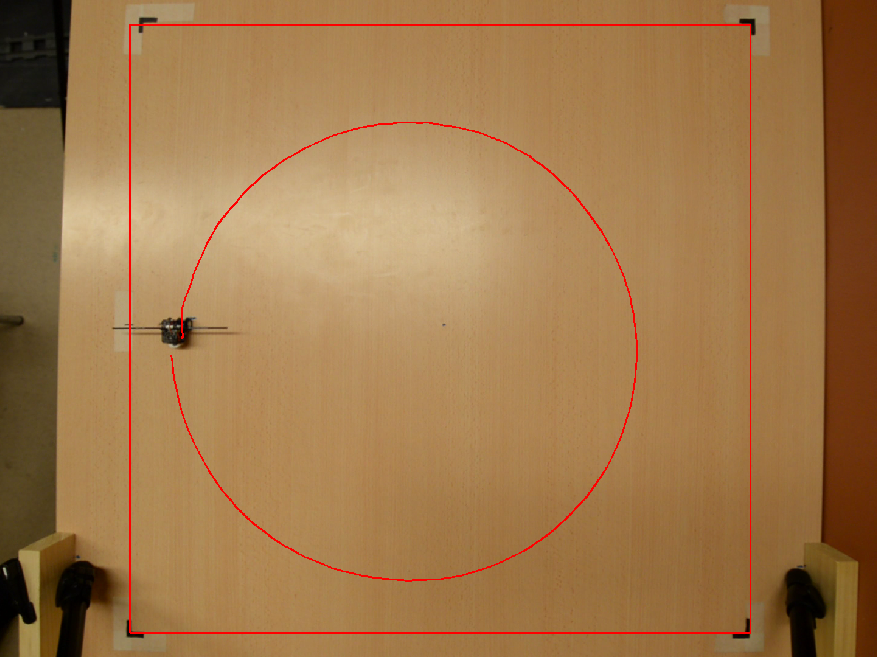
\includegraphics[width=\textwidth]{pics/movement_example.png}
		\caption{Tracking with OpenCV}
		\label{fig:movement_example}
	\end{subfigure}
	\caption{Experimental setup to record the robots movement}
\end{figure}


\subsection{Movement Accuracy Metrics}
The following metrics have been collected

\begin{itemize}
	\item average curvature of straight line movement
	\item Circle plot, make reference flat and plot difference between measured circle and reference (deviation from ideal circle for circular movements)
	\item for both straight and curved movements: length of the total movement and  standard deviation in length of movement
\end{itemize}


\subsection{Straight Movements}

The robot is commanded to move 75\,cm

\begin{figure}
	\centering
	\begin{subfigure}[b]{0.62\textwidth}
		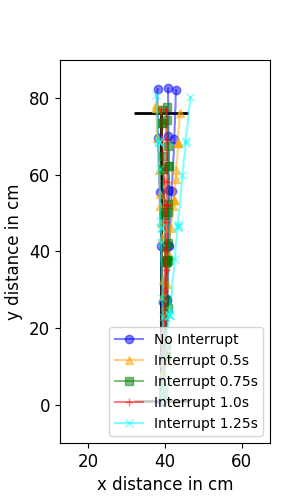
\includegraphics[width=\textwidth]{pics/straight_40.png}
		\caption{Target 40\%}
		\label{fig:stra_exp1}
	\end{subfigure}
	\begin{subfigure}[b]{0.62\textwidth}
		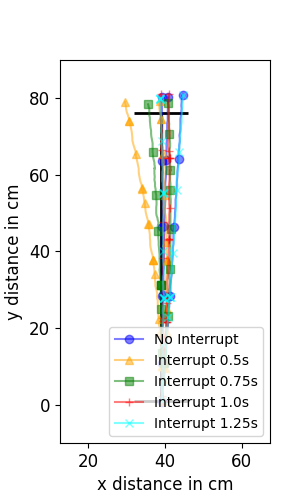
\includegraphics[width=\textwidth]{pics/straight_65.png}
		\caption{Target 65\%}
		\label{fig:stra_exp2}
	\end{subfigure}
	\begin{subfigure}[b]{0.62\textwidth}
		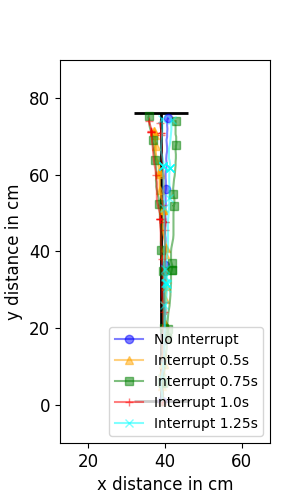
\includegraphics[width=\textwidth]{pics/straight_90.png}
		\caption{Target 90\%}
		\label{fig:stra_exp3}
	\end{subfigure}
	\caption{Straight movements, black horizontal lines show the begin and endpoints}
\end{figure}


\subsection{Circular Movements Results}

The robot is commanded make a circle with radius of 30\,cm


\begin{figure}
	\centering
	\begin{subfigure}[b]{0.62\textwidth}
		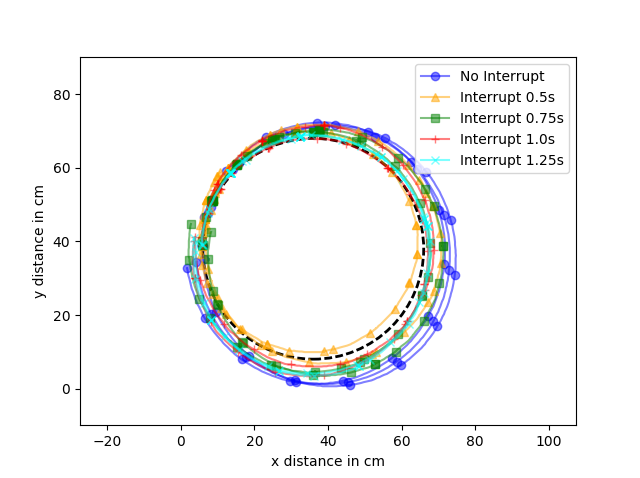
\includegraphics[width=\textwidth]{pics/circle_40.png}
		\caption{Target 40\%}
		\label{fig:circ_exp1}
	\end{subfigure}
	\begin{subfigure}[b]{0.62\textwidth}
		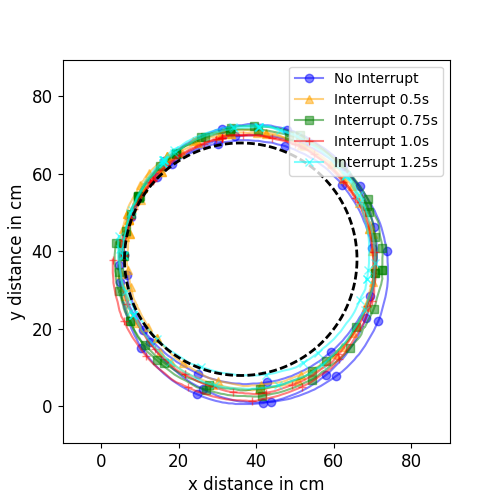
\includegraphics[width=\textwidth]{pics/circle_65.png}
		\caption{Target 65\%}
		\label{fig:circ_exp2}
	\end{subfigure}
	\begin{subfigure}[b]{0.62\textwidth}
		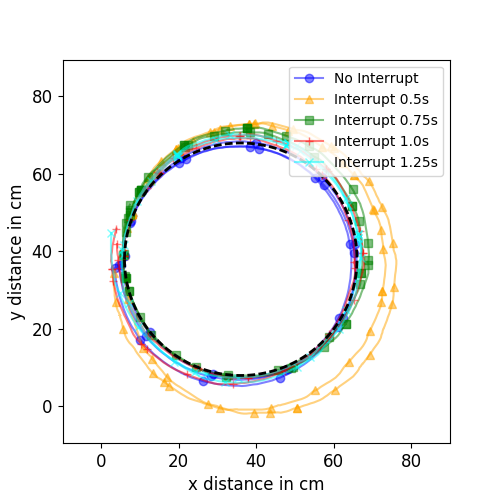
\includegraphics[width=\textwidth]{pics/circle_90.png}
		\caption{Target 90\%}
		\label{fig:circ_exp3}
	\end{subfigure}
	\caption{Circular movements, black dashed circle is the target}
\end{figure}


%\subsection{Results}
%Higher speed + more interrupts results in more drift to the left, because of wheel more in the back or weaker motor?
%How the interrupts are distributed over the distance has a influence or how the last interrupt ends up..
%Lower speed and less interrupts results in a higher accuracy??


%For square: Turn\_right speed should be high enough to turn within 0.5 sec

